\documentclass[12pt,oneside]{article}
\usepackage{light}
\usepackage{multicol}
\usepackage{pifont} % for the star
\usepackage{palatino}
\usepackage{mathpazo}
\usepackage{verbatim}

\newcommand{\mfigure}[3]{\bigskip\centerline{\resizebox{#1}{#2}{\includegraphics{#3}}}\bigskip}
\newcommand{\hint}[1]{({\it Hint: #1})}
\newcommand{\brule}[1]{\underline{\hspace{#1}}}
\newcommand{\ang}[1]{\left< #1 \right>}
\newcommand{\beats}{\rightarrow}


\newenvironment{falseproof}
{\begin{proof}[False proof]}
{\end{proof}}

\showsolutions
%\hidesolutions

\begin{document}
\generic{Midterm}{October 27, 2010}

\instatements{
\vspace{12pt}
\textbf{Name:} \rule{5in}{0.5pt}

\textbf{Circle the name of your recitation instructor}:

\begin{center}
\begin{tabular}{llllll}
David & Darren & Martyna & Nick & Oscar & Stav 
\end{tabular}
\end{center}

\begin{itemize}

\item This quiz is \textbf{closed book}, but you may have one $8.5
\times 11$'' sheet with notes in your own handwriting on both sides.

\item Calculators are not allowed.

\item You may assume all of the results presented in class.

\item Please show your work.  Partial credit cannot be given for a wrong
answer if your work isn't shown.

\item Write your solutions in the space provided.  If you
need more space, write on the back of the sheet containing the
problem.  Please keep your entire answer to a problem on that
problem's page.

\item Be neat and write legibly.  You will be graded not only on the
correctness of your answers, but also on the clarity with which you
express them.

\item If you get stuck on a problem, move on to others. The problems 
are not arranged in order of difficulty.

\item The exam ends at 9:30 PM.

\end{itemize}

\vspace{0.25in}

\begin{center}
{\large
\begin{tabular}{|c|c|c|c|}
\hline
Problem & Points & Grade & Grader \\ \hline \hline
1 & 10 & & \\ \hline
2 & 10 & & \\ \hline
3 & 20 & & \\ \hline
4 & 15 & & \\ \hline
5 & 20 & & \\ \hline
6 & 25 & & \\ \hline
7 & 10 & & \\ \hline
8 & 10 & & \\ \hline
Total & 120 & & \\ \hline
\end{tabular}
}
\end{center}
}
\instatements{\newpage}



\begin{problem}{10}

Consider these two propositions:
$$\texttt{P: } (A \vee B) \implies C$$
$$\texttt{Q: } (\neg C \implies \neg A) \vee (\neg C \implies \neg B)$$ 

Which of the following best describes the relationship between $P$ and $Q$?  Please circle exactly one answer.

\begin{enumerate}
\item
$P$ and $Q$ are equivalent
\item
$P \implies Q$
\item
$Q \implies P$
\item
All of the above
\item
None of the above
\end{enumerate}

Draw a truth table to illustrate your reasoning. You can use as many columns as you need.


\solution{

\begin{center}
{\large
\begin{tabular}{|c|c|c|c|c|}
\hline
A & B & C & P & Q \\ \hline
T & T & T & T & T \\ \hline
T & T & F & F & F \\ \hline
T & F & T & T & T \\ \hline
T & F & F & F & T \\ \hline
F & T & T & T & T \\ \hline
F & T & F & F & T \\ \hline
F & F & T & T & T \\ \hline
F & F & F & T & T \\ \hline
\end{tabular}
}
\end{center}

Observe from the last two columns of the table that $P \implies Q$ is always true, but $Q \implies P$ is not always true (e.g. line $4$).  Thus $P$ and $Q$ are not equivalent but $P \implies Q$. 

}

\end{problem}

\newpage


%%%%%%%%%%%%%%%%%%%%%%%%%%%%%%%%%%%%%%%%%%%%%%%%%%%%%%%%%%%%%%%%%%%%%%%%%%%%%%%%%%%%%%%%%%%%%%%%%%%%%%%% Strong Induction
\begin{problem}{10}

Let $G_0=1$, $G_1=3$, $G_2=9$, and define
\begin{equation}\label{Pn}
G_n =  G_{n-1} +3G_{n-2} + 3G_{n-3}
\end{equation}
for $n \geq 3$.  Show by induction that $G_n\leq 3^n$ for all $n \geq
0$.

\solution{

The proof is by strong induction with hypothesis $P(n) := G_n\leq 3^n$.

\begin{proof}
\textbf{Base Cases}

\textbf{$n=0$:} $G_0 = 1 = 3^0$.

\textbf{$n=1$:} $G_1 = 3 \le 3^1$.

\textbf{$n=2$:} $G_2 = 9 \le 3^2$.

\textbf{Inductive Step}:
Assume $n \geq 3$ and $P(k)$ for all $k$ such that $0 \leq k \leq n$.

\begin{align*}
G_{n}
& = G_{n-1} +3G_{n-2} + 3G_{n-3} & \text{by~\eqref{Pn}}\\
& \leq 3^{n-1} + (3)3^{n-2} + (3)3^{n-3} & \text{by induction hypothesis}\\
& = 3^{n-2} [3 + 3 + 1]\\
& = (7)3^{n-2}\\
& < (9)3^{n-2}\\
& = 3^{n} 
\end{align*}

\end{proof}
}
\end{problem}


\newpage

%%%%%%%%%%%%%%%%%%%%%%%%%%%%%%%%%%%%%%%%%%%%%%%%%%%%%%%%%%%%%%%%%%%%%%%%%%%%%%%%%%%%%%%%%%%%%%%%%%%%%%% squares and circles game
\begin{problem}{20}
%Taken from: http://www.cut-the-knot.org/ctk/invariant.shtml

In the game of Squares and Circles, the players (you and your computer) start with a shared finite collection of shapes: some circles and some squares. Players take turns making moves. On each move, a player chooses any two shapes from the collection. These two are replaced with a single one according to the following rule:

A pair of identical shapes is replaced with a square. A pair of different shapes is replaced with a circle.

At the end of the game, when only one shape remains, you are a winner if the remaining shape is a circle. Otherwise, your computer wins. 

\bparts

\ppart{5}
Prove that the game will end.

\solution{

\begin{proof}

We use induction on the number of turns to prove the statement. Let $n$ be the number of shapes originally, and let P(k) be the proposition that if $0\leq k \leq n-1$ then after k turns, the number of remaining shapes is $n-k$. Thus the game ends after $n-1$ steps. 


{\bf Base case:} $P(0)$ is true by definition; the number of reamaining shapes after 0 turns is $n-0=n$, the original number of shapes. 

{\bf Inductive step:} Now we must show that  $P(k)$ implies $P(k+1)$ for all $k\geq 0$.  If $k>=n-1$, $P(k)$ implies $P(k+1)$  would always be true, since $P(k+1)$ would be trivially true. So we only need to prrove this for $k<n-1$. So assume for your inductive hypothesis that $P(k)$ is true, where $0 \leq k < n-1$; that is, after $k$ turns the number of remaining shapes in $n-k$. Since $k<n-1$, the number of remaining shapes is $n-k>1$. Hence there are at least 2 shapes to choose from and the game has not ended yet. In the k+1st turn either the computer will choose 2 shapes, or you will choose two shapes. In either case the two shapes chosen, will be replaced by exactly once. Hence the number of shapes remaining will be $n-k-2+1=  n-k-1 = n-(k+1)$ as desired. This proves that $P(k)$ implies $P(k+1)$ for all $k \geq 0$.

By the principle of induction, $P(k)$ is true for all $k \geq 0$.

Hence, by our inductve hypothes after n-1 turns, 1 shape remains, which by the problem definition implies the game ends. 
\end{proof}

}

\newpage

\ppart{15}
Prove that you will win if and only if the number of circles initially is odd.
 
\solution{

\begin{proof}

We use induction on the number of turns to prove the statement. Let $a$ be the number of circles initially, and let P(k) be the proposition that if $0\leq k \leq n-1$ then after k turns, the number of remaining ciircles is $a-2i$, for some nonnegative integer $i$. Thus if $a$ is odd initially, at turn $n-1$, when the game ends, $a-2i$ circles - an odd number - remain, and since there is only one shape remaining, there must be exactly 1 circle left, and you win.

{\bf Base case:} $P(0)$ is true by definition; the number of reamaining circles after 0 turns is $a-2*0 = a$, the original number of shapes. 

{\bf Inductive step:} Now we must show that  $P(k)$ implies $P(k+1)$ for all $k\geq 0$.  If $k>=n-1$, $P(k)$ implies $P(k+1)$  would always be true, since $P(k+1)$ would be trivially true. So we only need to prrove this for $k<n-1$. So assume for your inductive hypothesis that $P(k)$ is true, where $0 \leq k < n-1$; that is, after $k$ turns the number of remaining circles is $a-2i_1$. for some nonnegative integer $i_1$. Since $k<n-1$, the number of remaining shapes is $n-k>1$ (from part a), hence there are at least 2 shapes to choose from and the game has not ended yet. In the k+1st turn either the computer will choose 2 shapes, or you will choose two shapes. If the two shapes chosen are both squares, then they are replaced by a square, and the number of circles doe not change, and hence is still $a-2i_1$. If the two shapes chosen are both circles, then they are replaced by a square, and the number of circles gets decreased by 2, and is $a-2i-2=a-2(i+1)$. If one of the shapes chosen was a circle and the other was a square, they get replaced by a circle, and again the number of circles does not change and remains $a-2i$. Hence in all three transitions P(k+1) holds.  

By the principle of induction, $P(k)$ is true for all $k \geq 0$.

Hence, by induction when the game ends the parity of the number of circles is the same as the original parity of the number of circles. So you will win only if the number of circles to begin with was odd. 

\end{proof}

}

\eparts

\end{problem}

%%%%%%%%%%%%%%%%%%%%%%%%%%%%%%%%%%%%%%%%%%%%%%%%%%%%%%%%%%%%%%%%%%%%%%%%%%%%%%%%%%%%%%%%%%%%%%%%%%%%%%%%%%%%%%%%%%%%%%%%%%%%%%%% pulverizer / finding inverses
\newcommand{\card}[1]{\left|#1\right|}

%number theory

\newpage

\begin{problem}{15}
\bparts
\ppart{8}
Find a number $x \in \{0, 1, \ldots, 112\}$ such that $11x \equiv 1 \pmod{113}$.

\solution[\vspace{4.5in}]{
We can do this using the pulverizer.  Specifically, if we find a pair $(s, t)$ such that $11s + 113t = 1$, then we know that $11s \equiv 1 \pmod{113}$.
\[
\begin{array}{ccccrcl}
x & \quad & y & \quad & \rem(x,y) & = & x - q \cdot y \\ \hline
113 && 11 && 3  & = &   113 - 10 \cdot 11 \\
11 && 3 && 2   & = &   11 - 3 \cdot 3 \\
&&&&            & = &   11 - 3 \cdot (113 - 10 \cdot 11) \\
&&&&            & = &   -3 \cdot 113 + 31 \cdot 11 \\
3 && 2  && 1   & = &   3 - 2 \\
&&&&		& = & ( 113 - 10 \cdot 11) - (-3 \cdot 113 + 31 \cdot 18) \\
&&&&            & = &   (4 \cdot 113 - 41 \cdot 11) \\
\end{array}
\]
From the above work we see that $1 = 4 \cdot 113 - 41 \cdot 11$, and so
$-41\cdot 11 \equiv 1  \pmod{113}$. Therefore -41 is \emph{an} 
inverse of 113. However, it is not the \emph{unique} inverse of
113 in the range $\{1,\ldots,113\}$, which is given by $\rem(-41,113)=72$. So the multiplicative inverse of $11$ modulo $113$ is $72$.
}

\ppart{7}
Find a number $y \in \{0, 1, \ldots, 112\}$ such that $11^{112111} \equiv y \pmod{113}$
\hint{Note that $113$ is a prime.}

\solution{By Fermat's Theorem, since $113$ is prime and $113$ and $11$ are relatively prime, it must be that
\[11 \cdot 11^{111} \equiv 11^{113-1} \equiv 1 \pmod {113},\]
so $x \equiv 111 \pmod {113}$ (where x is defined as in part a).
As a result,
\[11^{112111} \equiv 11^{112\cdot 1000 + 111} \equiv {11^{112}}^{1000} \cdot 11^{111} \equiv 1^{1000} \cdot x \equiv x \equiv 72 \pmod {113},\]
so the answer is $72$.
}

\eparts
\end{problem}

\newpage

%%%%%%%%%%%%%%%%%%%%%%%%%%%%%%%%%%%%%%%%%%%%%%%%%%%%%%%%%%%%%%%%%%%%%%%%%%%%%%%%%%%%%%%%%%%%%%%%%%%%%%%%%%%%%% concrete graph problem

\newpage

\begin{problem}{20}

Consider the simple graph $G$ given in figure $1$.

\begin{figure}[h]
\caption{Simple graph G}
\begin{center}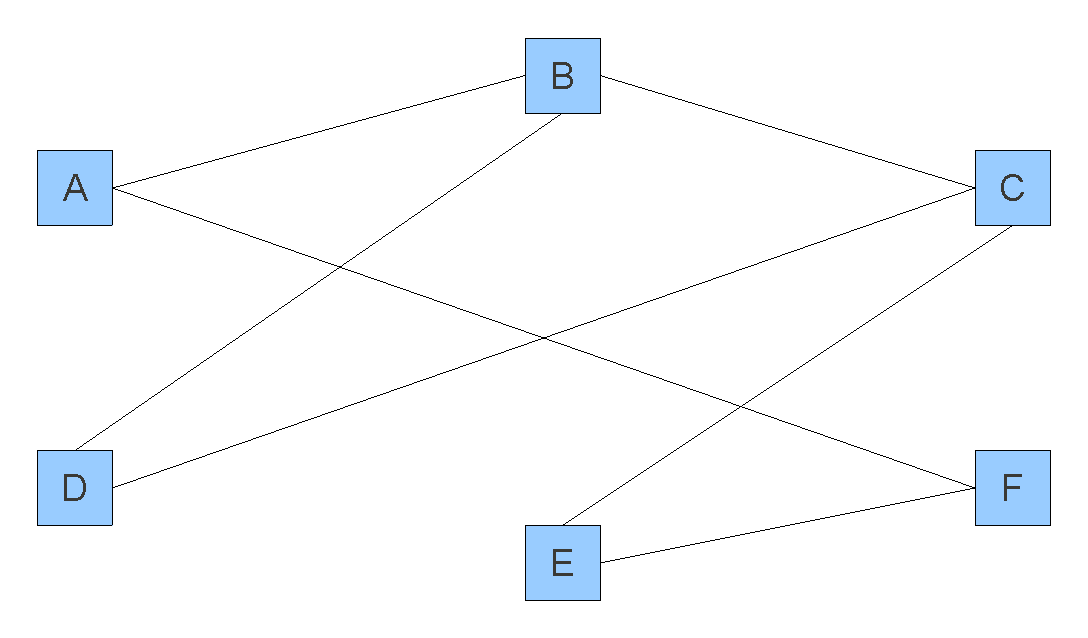
\includegraphics[width=12cm]{unweightedGraph.pdf}\end{center}
\end{figure}

\bparts

\ppart{4}
Give the diameter of $G$.
\solution[\vspace{2in}]{
Recall that the diameter is the maximum of all shortest path lengths between pairs of vertices.  Note that the shortest path length between $D$ and $F$ is $3$, and all other pairs of non-adjacent vertices share a neighbor.
}

\ppart{4}
Give a Hamiltonian Cycle on $G$.
\solution[\vspace{2in}]{
One possible solution is $(A, F, E, C, D, B, A)$.  This cycle and its reverse should constitute all possible solutions.
}

\newpage

\ppart{4}
Give a coloring on $G$ and show that it uses the smallest possible number of colors.
\solution[\vspace{3.5in}]{
One possible $3$-coloring is: $\{A, D, E\}$ red; $\{B, F\}$ green; $C$ blue.  Because there exists an odd-length cycle (e.g. $(B, D, C)$), no $2$-coloring exists.  Therefore the given coloring uses the least possible number of colors. 
}

\ppart{4}
Does $G$ have an Eulerian cycle?  Justify your answer.
\solution[\vspace{2in}]{No.  This follows from the fact that there exist vertices with odd degree; e.g. $B$.}

\eparts


\newpage

Now consider graph $H$, which is like $G$ but with weighted edges, in figure $2$:

\begin{figure}[h]
\caption{Weighted graph H}
\begin{center}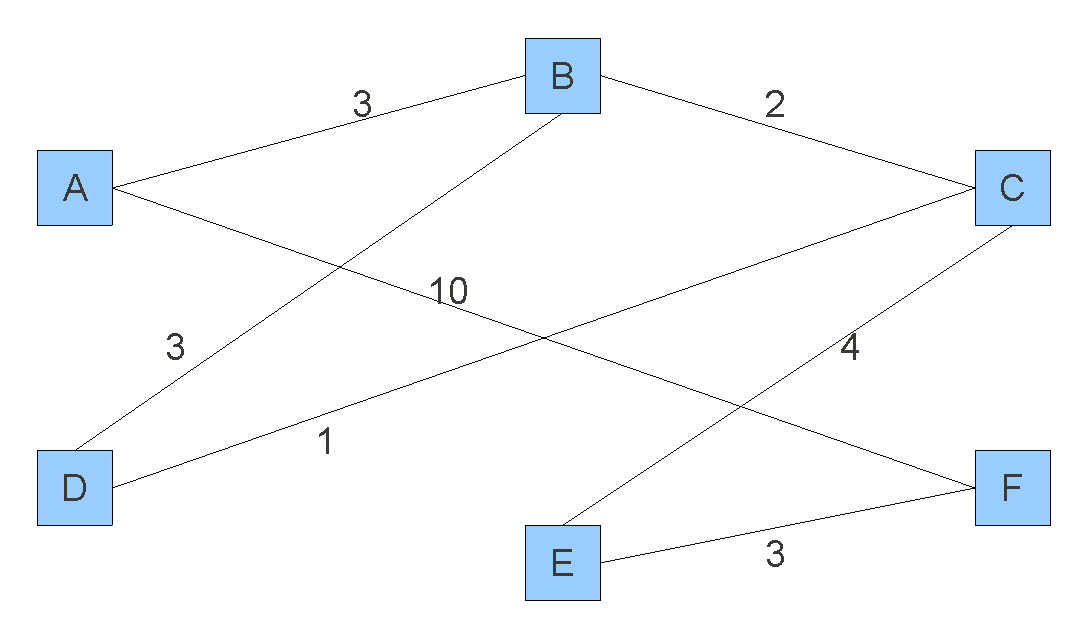
\includegraphics[width=12cm]{weightedGraph.pdf}\end{center}
\end{figure}

\bparts

\ppart{4}
Give a list of edges reflecting the order in which one of the greedy algorithms presented in class (i.e. in lecture, recitation, or the course text) would choose edges when finding an MST on $H$.
\solution[\vspace{2in}]{
Kruskal's alg (building up an acyclic subgraph) gives two possible orders: $((C,D), (B,C), (A,B), (E,F), (C,E))$ and $((C,D), (B,C), (E,F), (A,B), (C,E))$.  Prim's algorithm (building up a connected, acyclic subgraph) gives one possible order: \\ 
$((C,D), (B,C), (A,B), (C,E), (E,F))$.  Figure $3$ below gives the MST generated in any case.

\begin{figure}[h]
\caption{MST on graph H}
\begin{center}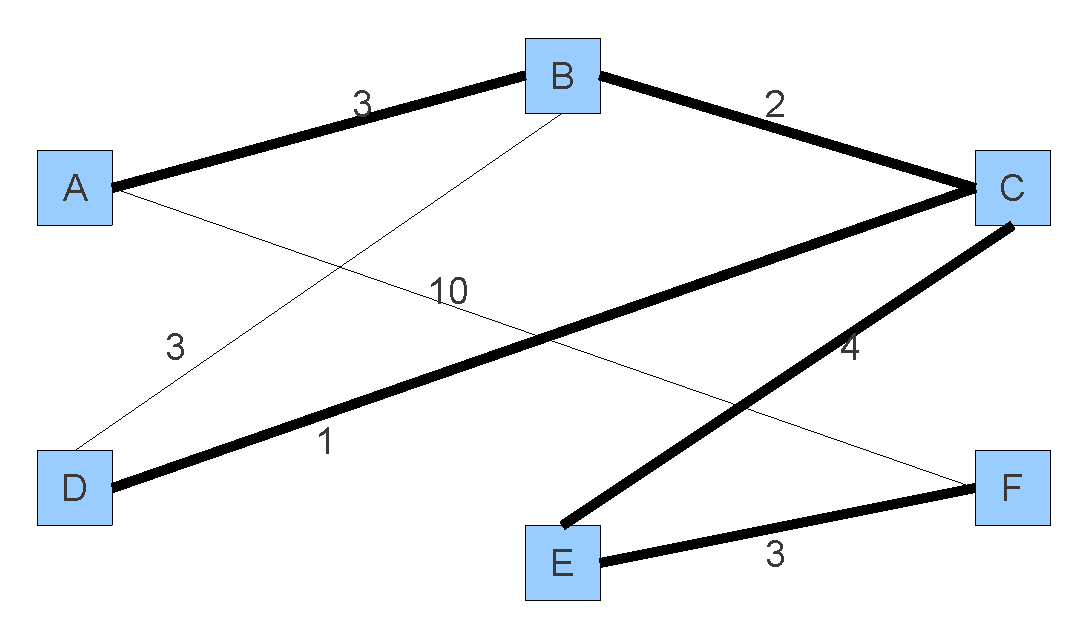
\includegraphics[width=12cm]{mstGraph.pdf}\end{center}
\end{figure}

}

\eparts
\end{problem}

\newpage

%%%%%%%%%%%%%%%%%%%%%%%%%%%%%%%%%%%%%%%%%%%%%%%%%%%%%%%%%%%%%%%%%%%%%%%%%%%%%%%%%%%%%%%%%%%%%%%%%%%%%%%%%%%%%%%% graph induction on edges
\newpage

\begin{problem}{25}
Let G be a graph with $m$ edges, $n$ vertices, and $k$ components. Prove that $G$ contains at least $m - n + k$ cycles. (Hint: Prove this by induction on the number of edges, $m$)

\solution{
The proof is by induction on m with hypothesis P(n):= If G is a graph with $n$ vertices, $m$ edges and $k$ components, then $G$ contains at least  $m + k -n = c$ cycles

\begin{proof}

\textbf{Base Case}
$m=0$: Let G be any graph with 0 edges and $n$ vertices. Then since there are no edges,  each vertex is its own connected component, hence there are $k=n$ connected components. Since there are no edges there are also no cycles. Lastly we note that $m+k-n=n+0-n=0$, and hence our base case. 

\textbf{Inductive Step}
Assume that P(m) holds, that is any graph with $m$ edges, $n$ vertices, and $k$ components has at least $m-n+k$ cycles. We must show that P(m+1) holds.

Consider an arbitrary graph $G$ with $m+1$ edges, $n$ vertices, and $k$ components. Suppose we remove an arbitrary edge, $e$, from $G$ to obtain $G'$. This edge, $e$, was either in a cycle in G or not:

\textit{Case 1:} $e$ is part of a cycle in $G$

If $e$ is in a cycle in $G$ then removing it removes at least one cycle. Furthermore, removing $e$ does not disconnect the graph so the number of components remains the same. So $G'$ has $m$ edges, $n$ vertices, and $k$ components, which by the inductive hypothesis tells us it has at least $m+k-n$ cycles. But $G$ has at least one more cycle than $G'$ (since $e$ is part of a cycle). So $G$ has at least $m+k-n +1$, or $(m+1)+k-n$ cycles, as desired.

\textit{Case 2:} $e$ is not part of a cycle in G
If $e$ is not part of a cycle removing it disconnects the graph of G, so the number of components in $G'$ is $k+1$. So, $G'$ contains $m$ edges, $n$ vertices, and $k+1$ components, so by the inductive hypothesis it contains at least $m+(k+1)-n$ cycles. Now since $e$ was not part of a cycle, $G$ and $G'$ have the same number of cycles. So $G$ also has at least$m+(k+1)-n$ cycles. Rearranging we get that $G$ has at least $(m+1)+k-n$ cycles as desired.

\end{proof}
}

\end{problem}

\newpage

%%%%%%%%%%%%%%%%%%%%%%%%%%%%%%%%%%%%%%%%%%%%%%%%%%%%%%%%%%%%%%%%%%%%%%%%%%%%%%%%%%%%%%%%%%%%%%%%%%%%%%%%%%%%%%%%%%%%%%%%%%%%%%%%%%% bounding sums

\begin{problem}{10}
For the following sum, find an upper and a lower bound that differ by at most $1$.
%
\[
\sum_{i=1}^{\infty} \frac{1}{\sqrt{i^3}}
\]
\solution{

To find the upper bound, we use the integral method, where $f(i)= \frac{1}{\sqrt{i^3}}$:
\begin{align*}
\sum_{i=1}^{\infty} \frac{1}{\sqrt{i^3}} & \leq f(1)+ \int_{1}^{\infty} \frac{1}{\sqrt{i^3}} dx \\
& = 1 - 2\frac{1}{\sqrt{i}} \Big |_{1}^{\infty} \\
& = 1 - 2\left(0 - 1\right) = 3\\
\end{align*}
To find the lower bound, we use also use the intergral method:
\begin{align*}
\sum_{i=1}^{\infty} \frac{1}{\sqrt{i^3}} & \geq \lim_{x\rightarrow \infty} \frac{1}{\sqrt{i^3}} + \int_{1}^{\infty} \frac{1}{\sqrt{i^3}} dx \\ 
&= 0+2 = 2\\
\end{align*}
The two bounds differ by exactly $1$. We conclude that
\[
2 \leq \sum_{i=1}^{\infty} \frac{1}{\sqrt{i^3}} \leq 3.
\]
}
\end{problem}


\newpage

%%O notation problem (Oscar) %%%%%%

\begin{problem}{10}
State whether each of the following claims is True or False and prove your answer.

\bparts
\ppart{2}
$x \ln{x}$ is $O\left( x \right)$
\solution[\vspace{4in}]{False. $\lim_{x \to \infty} x\ln{x}/x = \lim_{x \to \infty} \ln{x} = \infty > 0$}


\ppart{2}
$x/100$  is $o\left( x \right)$
\solution[\vspace{4in}]{False. In this case we have $\dfrac{x/100}{x} = \dfrac{1}{100} \to 1/100  > 0$ as $x \to \infty$}

\newpage
\ppart{2}
$x^{n+1}$ is $\Omega \left( x^n \right)$
\solution[\vspace{4in}] {True. Taking the quotient we arrive to  $ \dfrac{x^{n+1}}{x^n} = x \to \infty > 0 $} 

\ppart{4}
$n!$ is $\Theta \left( n^n \right)$.
\eparts

\solution[\vspace{4in}]{False. Stirling's formula asserts $n! \sim \dfrac{n^n \sqrt{2\pi n}}{e^n}$ so $\lim_{n \to \infty} n!/n^n = \lim_{n \to \infty} \dfrac{n^n \sqrt{2\pi n}}{n^ne^n} = \lim_{n \to \infty} \dfrac{\sqrt{2 \pi n}}{e^n} = 0 $. Hence $n!$ is not $\Theta \left( n^n \right)$.}

\end{problem}


\newpage

\begin{center}
(Notes)
\end{center}

\newpage

\mbox{}

\newpage

\mbox{}

\end{document}
